\clearpage
\section{Trigger}
\label{sec:trigger}

Events in the \gls{sr}, as well as events in all \glspl{cr}, were collected using a set of triggers based on missing transverse energy \MET (or {\tt MET}) and missing hadronic transverse momentum \mht (or {\tt MHT}), denoted by the HLT paths 
%a set of \ptmiss- and \hardmet-based triggers, denoted by the HLT paths

\begin{itemize}
\item
  \texttt{HLT\_PFMETX\_PFMHTX\_IDTight\_v* (X=90,100,110,120,130,140)} and
\item \texttt{HLT\_PFMETNoMuX\_PFMHTNoMuX\_IDTight\_v* (X=90,100,110,120,130,140)}.
\end{itemize}

Here, \texttt{X} indicates the threshold applied to the online \MET and \mht, as calculated by the \gls{pf} algorithm; the asterisks indicate that more than one version of the same trigger may have been used. During periods of higher instantaneous luminosity, trigger paths with lower thresholds became prescaled to reduce the
event rate; in such cases, the search relies on the higher-threshold triggers, which remained un-prescaled throughout all data-taking periods. To compensate for losses in efficiency associated with the higher trigger thresholds,  
a set of back-up triggers was used when the  low-threshold \MET-\mht triggers became prescaled:

\begin{itemize}
\item \texttt{HLT\_PFMETX\_PFMHTX\_IDTight\_PFHT60\_v* (X=100,110,120,130,140)},
\item \texttt{HLT\_PFMETNoMuX\_PFMHTNoMuX\_IDTight\_PFHT60\_v* (X=100,110,120,130,140)},
\item \texttt{HLT\_PFMET120\_PFMHT120\_IDTight\_HFCleaned\_v*},
\item \texttt{HLT\_PFMET120\_PFMHT120\_IDTight\_PFHT60\_HFCleaned\_v*}, and
\item \texttt{HLT\_PFMETNoMu120\_PFMHTNoMu120\_IDTight\_HFCleaned\_v*}.
\end{itemize}

The logical OR of all of the above trigger paths was taken as the online criterion for selecting events throughout the three years of
data-taking.  The efficiency of the trigger decision is estimated in a single-electron CR collected the single-electron trigger path
\begin{itemize}
\item \texttt{HLT\_Ele27\_WPTight\_Gsf\_v*}.
\end{itemize}
The efficiency is estimated as
\begin{equation}
\epsilon = \frac{ n_{\text{ev}}(\text{passing \MET-\mht trigger in reference sample}) }{n_{\text{ev}}(\text{reference sample})},
\end{equation}
where the reference sample corresponds to events passing the electron trigger and additionally required to have an offline electron with $\pt>30$ GeV and $|\eta|<2.4$ passing the Medium WP. The efficiency is shown as a function of offline analysis observables \mht and \njets in Figure~\ref{fig:main-trigger-real-met}.

\begin{figure}[]
\centering
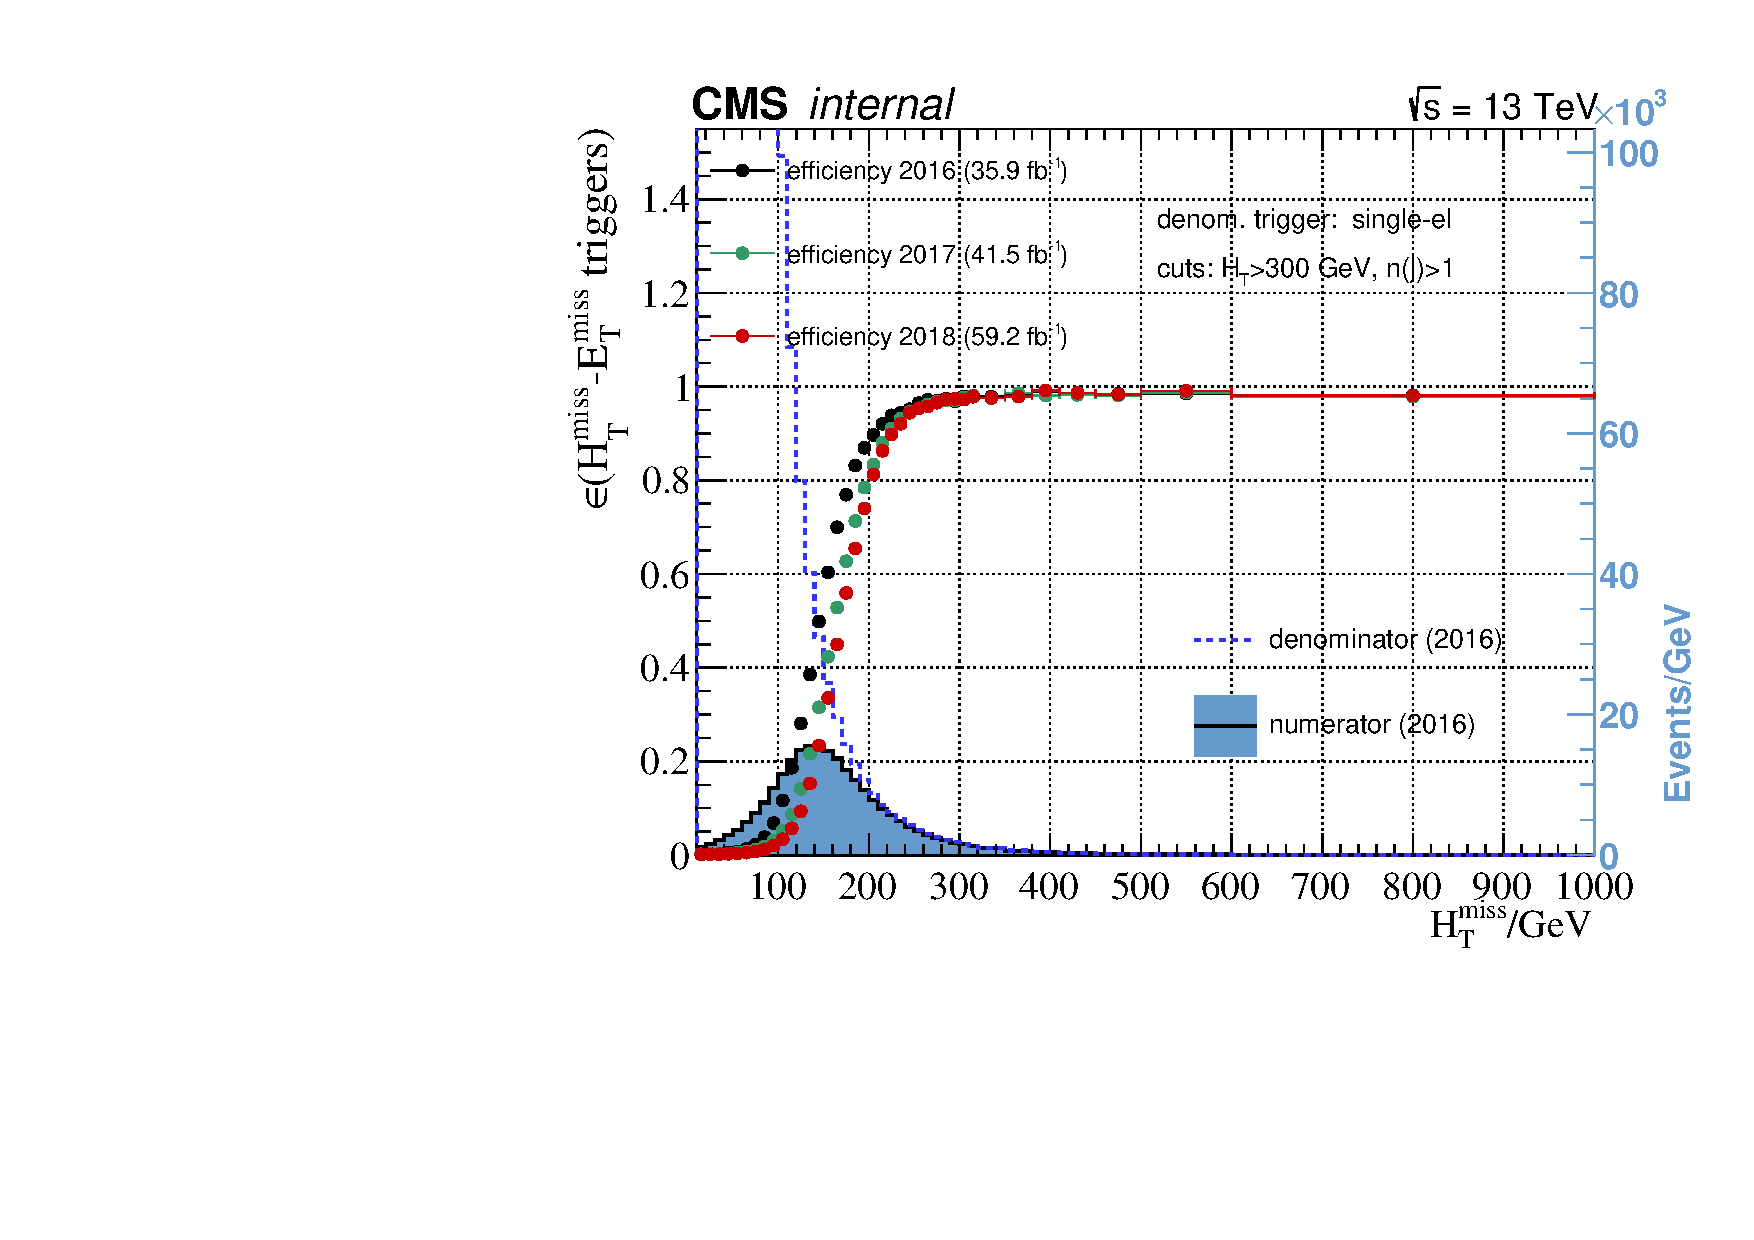
\includegraphics[width=0.48\linewidth]{plots/trigger/TrigEffMht.pdf}
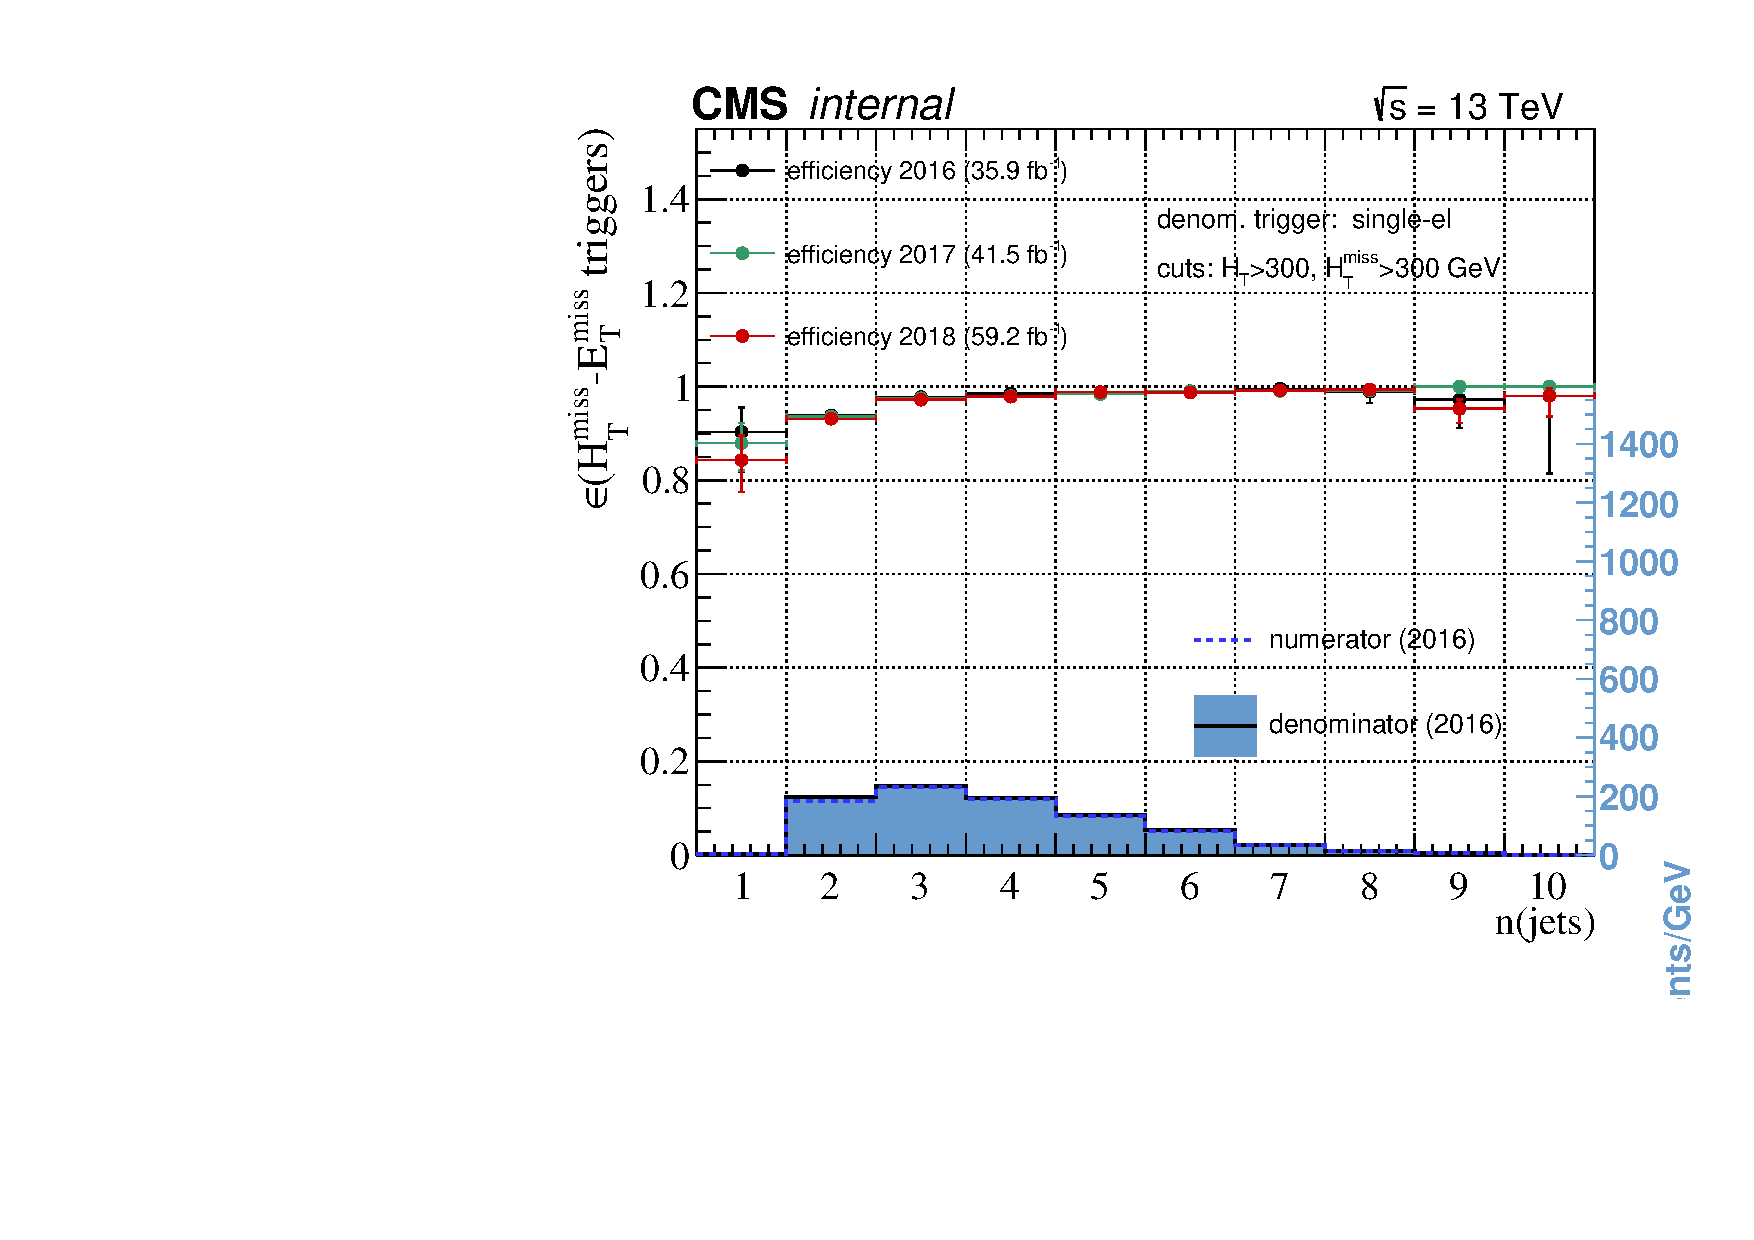
\includegraphics[width=0.48\linewidth]{plots/trigger/TrigEffNJets.pdf}
\caption{The efficiency of the set of \MET-\mht cross triggers measured in a single-electron control region, shown for \mht (left) and number of jets (right). The jet multiplicity is shown for \mht$>300$ GeV to account for the trigger turn-on.
  % This trigger set used to collect events in the signal region as well as the   single-lepton and QCD validation control  regions.
  %The measured efficiency is applied as an event weight to simulated signal events.
  }
\label{fig:main-trigger-real-met}
\end{figure}

The trigger efficiency has been studied previously, e.g., in SUS-19-006~\cite{CMS-PAS-SUS-19-006}, the efficiency measured in the SingleElectron datastream is consistent with the efficiency corresponding to SUSY signal events. The efficiency is applied as event weights extracted from the binned efficiency shown in Figure~\ref{fig:main-trigger-real-met}.



